\documentclass[a4paper,11pt]{article}

	%% From https://github.com/aytchell/latex-listings-protobuf/tree/09c39676e6afb2af8c7d21ed21a516359c52e27c/

\usepackage{xcolor}
\usepackage{xcolor-solarized}
\usepackage{textcomp}

\newcommand{\SetProtoColorsSolarized}{
  % Colors taken from the 'solarized' color scheme of Ethan Schoonover
  % (with light background)
  % http://ethanschoonover.com/solarized
  \colorlet{proto_basic}{solarized-base00}
  \colorlet{proto_keyword}{solarized-cyan}
  \colorlet{proto_type}{solarized-cyan}
  \colorlet{proto_options}{solarized-cyan}
  \colorlet{proto_comment}{solarized-base1}
  \colorlet{proto_string}{solarized-blue}
  \colorlet{proto_number}{solarized-violet}
  \colorlet{proto_ident}{solarized-base00}
  \colorlet{proto_digits}{solarized-violet}
  \colorlet{proto_background}{solarized-base3}
}

\newcommand{\SetProtoColorsBlueish}{
  % Colors inspired by the NASM style of Robin Eklind
  % https://github.com/mewspring/latex
  \definecolor{proto_basic}{RGB}{0,0,0}             % black
  \definecolor{proto_keyword}{RGB}{0,0,0}         % black
  \definecolor{proto_ident}{RGB}{128,0,0}            % dark red
  \definecolor{proto_options}{RGB}{128,0,128}       % purple
  \definecolor{proto_comment}{RGB}{0,128,0}         % dark green
  \definecolor{proto_string}{RGB}{255,0,0}          % red
  \definecolor{proto_number}{RGB}{108,113,196}      % violet
  \definecolor{proto_type}{RGB}{0,0,255}             % blue
  \definecolor{proto_digits}{RGB}{0,0,128}          % dark blue
  \definecolor{proto_background}{RGB}{255,255,255}  % white
}

\newcommand{\SetProtoColorsTomorrow}{
  % Colors taken from the 'Tomorrow' color scheme of Chris Kempson
  % https://github.com/chriskempson/tomorrow-theme/blob/master/vim/colors/Tomorrow.vim
  \definecolor{proto_basic}{RGB}{77, 77, 76}          % dark grey
  %\definecolor{proto_keyword}{RGB}{245, 135, 31}      % orange
  \definecolor{proto_keyword}{RGB}{66, 113, 174}      % orange
  %\definecolor{proto_type}{RGB}{66, 113, 174}         % purple
  \definecolor{proto_type}{RGB}{200, 40, 41}         % red
  \definecolor{proto_options}{RGB}{137, 89, 168}
  %\definecolor{proto_comment}{RGB}{142, 144, 140}     % gray
  \definecolor{proto_comment}{RGB}{0,0,0}             % black
  \definecolor{proto_string}{RGB}{113, 140, 0}        % green
  \definecolor{proto_number}{RGB}{137, 89, 168}
  %\definecolor{proto_ident}{RGB}{200, 40, 41}         % red
  \definecolor{proto_ident}{RGB}{0,128,0}           % dark green
  \definecolor{proto_digits}{RGB}{245, 135, 31}       % orange
  \definecolor{proto_background}{RGB}{255, 255, 255}  % white
}

%\SetProtoColorsSolarized{}
\SetProtoColorsTomorrow{}
%\SetProtoColorsBlueish{}

\lstdefinestyle{protobuf}{
  frame=lines,
  %xleftmargin=\parindent,
  belowcaptionskip=1\baselineskip,
  backgroundcolor=\color{proto_background},
  basicstyle=\color{proto_basic}\footnotesize\ttfamily,
	keywordstyle=[1]\color{proto_keyword},
	keywordstyle=[2]\color{proto_type},
	keywordstyle=[3]\color{proto_options},
	commentstyle=\color{proto_comment},
	stringstyle=\color{proto_string},
  numberstyle=\color{proto_ident}\tiny,
  identifierstyle=\color{proto_ident}\bfseries,
	numbers=none, %left,
	numbersep=5pt,
	breaklines=false,
	showstringspaces=false,
	tabsize=2,
	prebreak=\raisebox{0ex}[0ex][0ex]{\ensuremath{\hookleftarrow}},
	upquote=true,
}

	
        \usepackage[notes=true]{dtrt}
	\usepackage{algorithm}
	\usepackage{algpseudocode}
	\usepackage{amsmath}
	\usepackage{xcolor}
	\usepackage{graphicx}
	\usepackage{todonotes}
	\usepackage{listings}
	\usepackage{pxfonts}
	\usepackage[margin=1in]{geometry}

	\usepackage{lib/lang}  % include language definition for protobuf
	\usepackage{lib/style} % include custom style for proto declarations.	
	
	%\usepackage{sagetex}

	% Auuthor notes (using dtrt's macros). Switch the dtrt package flag to notes=false to hide.
	\definecolor{darkgreen}{rgb}{0,0.6,0}
	\newcommand{\dnote}[1]{\dtcolornote[Daniel]{red}{#1}}
	\newcommand{\anote}[1]{\dtcolornote[Aurell]{blue}{#1}}
	\newcommand{\enote}[1]{\dtcolornote[Eran]{darkgreen}{#1}}

	\newcommand\dtodo[1]{\todo[color=red!20]{#1}}
	\newcommand\atodo[1]{\todo[color=green!20]{#1}}
	\newcommand\etodo[1]{\todo[color=blue!20]{#1}}
	\def\boxit#1{%
		\smash{\color{red}\fboxrule=1pt\relax\fboxsep=-2pt\llap{\rlap{\fbox{\strut\makebox[#1]{}}}~}}\ignorespaces
	}
	
	%\makeatletter
	%\def\BState{\State\hskip-\ALG@thistlm}
	%\makeatother
	
	%opening
	\title{zkInterface, a tool for zero-knowledge interoperability}
	\author{Daniel Benarroch, Kobi Gurkan, Aurel Nicolas, Eran Tromer}
	
	\begin{document}
		
		\maketitle
		
		\enote{Add abstract}

%=============================================================================
\section{Overview}

%-----------------------------------------------------------------------------
\subsection{Background}
\enote{Rewrite:}
Implementing zero-knowledge proof constructions is not a trivial task and comes with diverse matters, as is extensively explained in the \href{https://zkproof.org/proceedings-snapshots/zkproof-implementation-20180801.pdf}{Implementation Track proceeding} of the first ZKProof workshop. One of the requirements is to create a compiler of programs into constraint systems that are consumed by the proving system.

There are several trade-offs one can consider when designing general-purpose (front-end) compilers, leading to distinct frameworks, APIs, generality, etc. Today, existing compilers are implemented to work best with their corresponding (back-end) proving system (somemetimes more than one). For a comprehensive list of front-ends and back-ends, you can go to \href{https://zkp.science}{zkp.science}. 

These libraries are usually built end-to-end: they take in some program that defines the statement and generate or verify a proof, in many cases without explicitly exposing the constraint system compilation. Moreover, if the compilers can output intermediary files and configurations, they are usually native to the specific back-end. In practice this means that
\begin{itemize}
	\item there is no portability between different proving systems and compilers, and
	\item it is not possible to compile a program using code from different frameworks
\end{itemize}   

%-----------------------------------------------------------------------------
\subsection{Goals}
\enote{Rewrite:}

\enote{Copy relevant text from the Implementation Track, especially Advanced Interoperability}

We aim to solve this issue, as seen in Figure \ref{interface}, by creating a community standard proposal for the ZKProof effort around constraint system formatting, building upon the work done at the first ZKProof workshop.

We design and implement a standard rank-1 constraint system (R1CS) interface between front-ends and back-ends. Our design encompasses programmable instance and witness reductions, while capturing the parameters of the different components of the statement to be proven. Given that these statements can be large and difficult to build, developers usually build smaller components that are re-usable with different statements; these components are sometimes called ``gadgets". With our zkInterface one can piece together programmatically the different components to form a complete statement.

\paragraph{Desiderata}
\begin{itemize}
	\item Interoperability across frameworks and programming languages
	\item The ability to write components that can be consumed by different frameworks
	\item Overhead of the R1CS construction and witness reduction should be linear compared to a native implementation of the same gadgets 
	\item Design an extensible interface, for example to support non R1CS systems.
\end{itemize}

\paragraph{Scope and limitations.} \enote{Rewrite:}

We aim for the standard interface to be as generic as possible, including non-R1CS-based proving systems. However, the current proposal is more limited, mainly due to time constraints.

The standard that we propose can be seen in three different levels:
\begin{enumerate}
	\item The first level defines  
	\begin{itemize}
		\item standard messages and their serialization that the caller and callee exchange, 
		\item an R1CS file format for the instance
		\item a file format for the assignments.
	\end{itemize}
	\item The second level defines a simple C API that allows for the exchange of messages.
	\item The third level defines the self-contained packaging of a component for its portable execution on different platforms.
\end{enumerate}

This proposal is not aiming to standardize a language or framework for generating constraint systems, nor the way that components of the proving statement should be written. However, it is important to point that any such framework could use the proposed interface.

\section{Description}
		
		zkInterface is a purely functional interface for zero-knowledge systems that enables cross-language interoperability via dynamic linking and shared memory. The current version, even if limiting, creates an interface based on R1CS formatting and offers the ability to abstractly craft a constraint system building from different components, possibly written in different frameworks, by determining how data should be written and read. 
		
		It can also be seen as a design tool for improved generation of constraints and usability, analogous to a portable binary format, since one can parametrize the functions calls and easily compose different functions, or components, that are not directly compatible.
		
		It is important to point out that the interface can be called both to write a request or read a response by having an encoder at the front-end  and a decoder at the back-end. 
		
		\paragraph{Main functionality.}
		
		The interface works across every zero-knowledge front-end and back-end, minimizing, when possible, the overhead of using a general format. This is achieved in several ways:
        
        \begin{itemize}
			\item By using a protoboard-like method for shared memory allocation, and thus preventing double-copying the data unnecessarily.
			\item By parametrizing the function calls to the different components so to take advantage of the specific context underlying those components.
			\item By using FlatBuffers, an efficient cross platform serialization library for different languages. This tool allows us to easily write ad-hoc parsers from scratch and has a very low overhead in shared memory, which can be used in regular function calls. 
		\end{itemize}
		
		
        
        The two main purposes of the interface are the computations of the \emph{instance reduction}, which generates a portable circuit or constraint system, and the \emph{witness reduction}, which assigns values to the variables allocated in the instance reduction. We have designed the interface so that each of these two processes actually use the same exact routine, except with different message types.

        Essentially, as seen in Figure \ref{flow}, the caller of the interface can be both an application or a component that requires a sub-component, an abstraction that helps make the interface minimal. Say I want to compute a proof of set membership by using a Merkle Tree of hashes. Then, the flow is the following:
        \begin{enumerate} 
            \item The application will call the Merkle Tree component that exists in some front-end framework, which starts allocating in memory the variables and constraints in the standard R1CS format.
            \item For every hash computation needed to generate the path, the Merkle Tree will itself call a hasher sub-component, possibly from a different framework, by passing it the parameters, including the next free memory slot for allocating the hash constraints and variables.
            \item The hash component will then allocate in memory the constraints and variables, to which the Merkle Tree component is oblivious (except the shared input / outputs: the input message and the output hash digest).
            \item Specifically, for each call to the hash component, the input message is given as part of the request and the hash component sends the hash digest as part of the response. The rest of the variables are locally dealt with by the hash component but are shared in memory by all the components.
        \end{enumerate}
        
        Note how the routine can be re-used by the witness reduction and deterministically assign the values to the respective variables in memory. Moreover, if needed, the constraint system can be outputed as a file containing a static rank-1 constraint system. One objection to using this routine design is that the component at the top level (i.e.: the Merkle Tree) cannot is waiting for the response of the sub-component (i.e.: the hasher component). This can have a cost in the efficiency of the circuit generation if we imagine a long enough chain of sub-calls that would cause a quadratic overhead. This is unlikely to happen in the current set of applications and circuits. \dtodo{Please check that this is true}
		
			\begin{figure}[h!]
				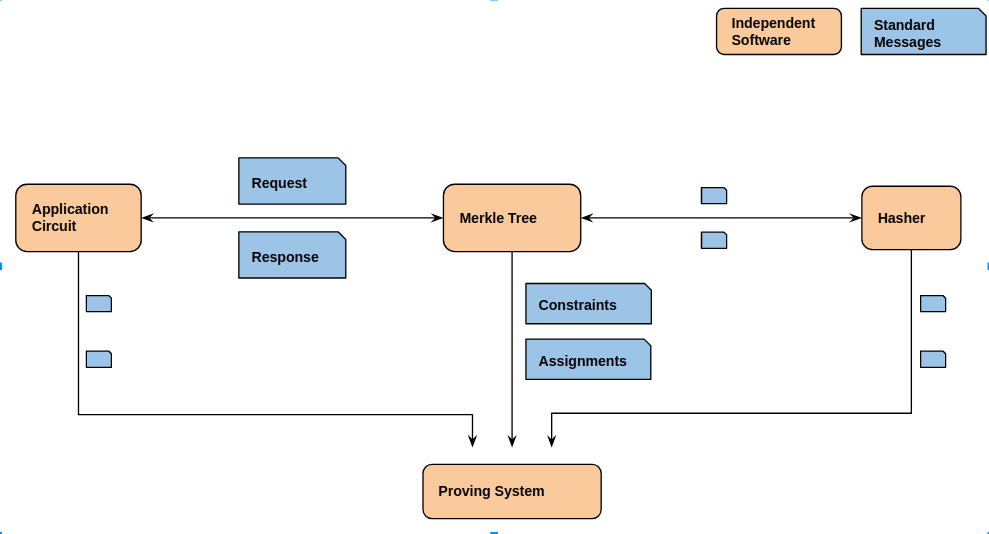
\includegraphics[width=\linewidth]{routine.png}
				\caption{The flow of interaction between existing libraries and the interface}
				\label{flow}
			\end{figure}

		\paragraph{Instance reduction.} 
		
        Points to include:
        - caller does not provide functionality to gadget and does not depend on specific implementation
        - gadget and caller both allocate variables
		
		\paragraph{Witness reduction.}
		
		r1cs in the format: a way to represent the constraints and a way to represent the assignment; and connection between components (gadgets), which actually are the public inputs. If we think of circuit as components, each component has a set of local inputs and "outgoing" inputs.
		
		So the interface solves two problems: 1/ interop between frameworks (front-ends) and proving systems (backends) 2/ composability of gadgets between different frameworks.
		
	
		
		\subsection{An MVP}
		
		
		
		\subsection{Specification}
        
        \paragraph{Interface Definition.}
        
        \paragraph{Request Call.}

        \paragraph{Callee Response.}

        \paragraph{Memory Allocation.}

        \paragraph{FlatBuffers.}

        \paragraph{Standard Format.}

		*use of flatboard
		
		- semantics; planned parametrization of the semantics.
		
		- format: can work with files (all messages instead of processing, can be written to file) for both instance / witness reduction, otherwise can work with memory 
		
		Each component has an interface; which can be invoked / instantiated / called with other components to make up the constraint system.
			- composibility of gadgets as there local variables / public ones (merkle tree has the leaf and root and invokes sha256)
		
		CRS is specific to proving system so the format does not handle the CRS portability
		
		we are thinking of implementing ZoKrates for the application layer and libsnark, bellman.  
		
		NOTE: some people think of functions, inputs and returned variables; others as circuits and gadgets.
		
		
		Issues: 1/ linear 

%=============================================================================
\section{Specification}

\enote{For now, maybe just remove this section, and leave only the narrative in the Architecture subsection, and the in-source comments?}
		
\paragraph{Interface Definition.}

	The interface is defined as a FlatBuffers schema that describes 
	the serialization of messages that the caller and callee can exchange.

	The FlatBuffers system includes a simple interface definition language,
	support for all common programming languages,
	a clear evolution path for future extensions of the standard,
	and the possibility of very efficient implementations.

	\anote{Add ref: https://google.github.io/flatbuffers/}

	The interface definition is provided in annex.

\paragraph{Request Call.}

\paragraph{Callee Response.}

	\paragraph{C API.}

\paragraph{Memory Allocation.}

\paragraph{File Format.}

\subsection{Interface Definition}



\lstinputlisting[language=flatbuffers2,style=protobuf]{../gadget.fbs}

	
\end{document}